% Paper 1 -- Fidetype. Draft v4: supplementary material (Sections S1-S24). Build after main.tex (see main.tex).
\documentclass[11pt,a4paper]{article}
% ---------------------------------------------------------------- CLASS (swap for IOP template)
\usepackage[a4paper,margin=2.5cm]{geometry}
\usepackage[T1]{fontenc}
\usepackage[utf8]{inputenc}
\usepackage{lmodern}
\usepackage{microtype}
% ---------------------------------------------------------------- packages
\usepackage{amsmath,amssymb}
\usepackage{graphicx}
\usepackage{booktabs}
\usepackage{adjustbox}
\usepackage{enumitem}
\usepackage{multirow}
\usepackage{array}
\usepackage{xcolor}
\usepackage{tikz}
\usetikzlibrary{arrows.meta,positioning,shapes.geometric,fit,calc,backgrounds}
\usepackage[font=small,labelfont=bf]{caption}
\usepackage{subcaption}
\usepackage{placeins}
\usepackage{float}
\usepackage{algorithm}
\usepackage{algpseudocode}
\usepackage[numbers,sort&compress]{natbib}
\usepackage{xr-hyper}
\usepackage[colorlinks=true,linkcolor=blue!50!black,citecolor=blue!50!black,urlcolor=blue!50!black]{hyperref}
\usepackage{url}
\usepackage[capitalise,noabbrev]{cleveref}

\graphicspath{{../figures/}}
\emergencystretch=2em

% ---------------------------------------------------------------- macros
% \todo{...}: visible red marker for missing data or open decisions. Never remove one
% without filling the gap it names. Grep "\todo" to list them.
\newcommand{\todo}[1]{\textcolor{red}{\textbf{[TODO: #1]}}}
\newcommand{\nts}{NeuralTextStream}
\newcommand{\ewpm}{eWPM}
\newcommand{\act}[1]{\textsc{#1}}
\newcommand{\code}[1]{\texttt{#1}}
\newcommand{\ci}[2]{\ensuremath{[#1,\,#2]}}  % math mode: "-0.11" prints a true minus sign
\newcommand{\papertitle}{When should a neural text-entry decoder commit?\\Risk-controlled commits from a stream-level trust layer}
% import only the labels of the main paper, not its citation numbers (each file has its own reference list)
\let\origbibcite\bibcite\def\bibcite#1#2{}
\externaldocument{build/main}
\let\bibcite\origbibcite
% generated table rows (make_supp_tables.py): primitive input, so that \midrule may follow inside a tabular
\makeatletter\newcommand{\inputrows}[1]{\@@input #1 }\makeatother

\renewcommand{\thesection}{S\arabic{section}}
\renewcommand{\thetable}{S\arabic{table}}
\renewcommand{\thefigure}{S\arabic{figure}}
\renewcommand{\thealgorithm}{S\arabic{algorithm}}
\renewcommand{\theequation}{S\arabic{equation}}

\title{Supplementary material for:\\[2pt] \papertitle}
\author{\todo{authors, affiliations, e-mail}}
\date{}

\begin{document}
\maketitle
\noindent References to Sections 1--9, Tables 1--4, Figures 1--3, Algorithm 1 and Appendix A point to the main paper. All numbers come from committed result files; the round-4 analyses are in \code{experiments/2026-11-12-paper1-r4-analyses/} of the repository.

\tableofcontents

% Supplementary material of Paper 1 (draft v4). Section, table, figure and algorithm numbers carry the prefix S.
% References to the main paper (sections, Tables 1-4, Figures 1-3, Algorithm 1) resolve through xr (main.aux).

\section{Notation}
\label{app:notation}

\begin{table}[H]
  \centering
  \caption{\textbf{Notation.} Prose uses ``error among commits''; tables use EAC.}
  \label{tab:notation}
  \small
  \begin{adjustbox}{max width=\linewidth}\begin{tabular}{@{}ll@{\qquad}ll@{}}
    \toprule
    \textbf{Symbol} & \textbf{Meaning} & \textbf{Symbol} & \textbf{Meaning} \\
    \midrule
    $F_i$, $V$ & frames in the stream of item $i$; vocabulary size & $\lambda$ & commit threshold on $s_i$ \\
    $K$ & candidate list size ($K = 10$; 11 for the published gate) & $s_i$ & commit score: $\hat p_{\mathrm{top1}}$ if eligible, else $-\infty$ \\
    $\hat p_{\mathrm{top1}}$ & calibrated probability of the top candidate & $c_i$ & 1 if the top candidate is wrong \\
    $\tau_f$, $\tau_s$ & frame and sentence temperatures & $L_i(\lambda)$ & loss $c_i\,\mathbf{1}[s_i \ge \lambda]$ \\
    $g_i$ & guard risk of the top candidate, in $[0,1]$ & $R(\lambda)$, $\hat R_n(\lambda)$ & population and calibration risk \\
    $r_{\mathrm{abst}}$, $r_{\mathrm{max}}$ & guard limits for abstain and commit & $n$ & number of calibration items \\
    $k$, $k_{\max}$ & offered candidates; offer limit & $\alpha$ & target wrong-commit rate (0.05) \\
    $q$ & conformal quantile of the sentence set & $\beta$ & target error among commits (0.10, 0.20) \\
    $n_\lambda$, $k_\lambda$ & calibration commits and wrong commits at $\lambda$ & $\delta$ & failure probability of LTT (0.1) \\
    $\eta$, $\gamma$ & step sizes of the online controllers & $T$, $d$ & items in an online sequence; feedback delay \\
    \bottomrule
  \end{tabular}\end{adjustbox}
\end{table}

\section{Fitting and calibration}
\label{app:algorithms}

\begin{algorithm}[H]
\caption{Fitting and calibration of the commit threshold}
\label{alg:calibrate}
\small
\begin{algorithmic}[1]
\Require fit items $\mathcal{F}$ (parts $\mathcal{F}_1$, $\mathcal{F}_2$, $\mathcal{F}_3$; see below), disjoint calibration items $\mathcal{C}$ ($n$ items with truth), $\alpha$, $\beta$, $\delta$
\State $\tau_f \gets \arg\min_\tau$ cross-entropy of the aligned true tokens at the greedy CTC peaks of $\mathcal{F}_1$ \Comment{golden section, $\tau \in [0.05, 20]$}
\State $\tau_s \gets \arg\min_\tau$ binary NLL of $[y_1 = \text{truth}]$ under $\mathrm{softmax}(\text{score}/\tau)_1$ on $\mathcal{F}_1$
\State $q \gets$ the $\lceil (m+1)(1 - 0.1)\rceil$-th smallest $1 - \hat p_{\text{truth}}$ over the $m$ items of $\mathcal{F}_2$ whose truth is in the $K$-best list
\State $(\lambda_{\mathrm{tuned}}, r_{\max}, r_{\mathrm{abst}}, k_{\max}, \text{fallback}) \gets$ grid point with the highest \ewpm{} on $\mathcal{F}_3$ among those with wrong-commit rate $\le \alpha$ (first in grid order on ties; if none, the lowest wrong-commit rate)
\State compute $s_i$ and $c_i$ for every $i \in \mathcal{C}$ (Algorithm~\ref{alg:decide} up to the commit score)
\State \textbf{CRC:} $\hat\lambda_{\mathrm{CRC}} \gets \min\{\lambda \in \{s_i\} \cup \{+\infty\} : (\sum_i c_i \mathbf{1}[s_i \ge \lambda] + 1)/(n+1) \le \alpha\}$
\State \textbf{LTT:} for $\lambda = 1.00, 0.99, \ldots, 0.00$: $k \gets \sum_i c_i \mathbf{1}[s_i \ge \lambda]$; if $\Pr(\mathrm{Bin}(n,\alpha) \le k) \le \delta$ then $\hat\lambda_{\mathrm{LTT}} \gets \lambda$ else stop \Comment{$+\infty$ if the first test fails}
\State \textbf{Max rule (primary):} $\lambda \gets \max(\lambda_{\mathrm{tuned}}, \hat\lambda_{\mathrm{LTT}})$ \Comment{CRC max rule: $\max(\lambda_{\mathrm{tuned}}, \hat\lambda_{\mathrm{CRC}})$}
\State \textbf{Joint LTT} (targets $\alpha$, $\beta$): for $\lambda \in \{0.05, 0.10, \ldots, 1.00\}$: $p_{\mathrm{marg}} \gets \Pr(\mathrm{Bin}(n,\alpha) \le n\hat R_n(\lambda))$, $p_{\mathrm{sel}} \gets \Pr(\mathrm{Bin}(n_\lambda,\beta) \le k_\lambda)$ (1 if $n_\lambda = 0$); reject if $\max(p_{\mathrm{marg}}, p_{\mathrm{sel}}) \le \delta/20$; $\hat\lambda_{\mathrm{joint}} \gets$ the smallest rejected $\lambda$ ($+\infty$ if none). \emph{LTT-sel}: the same with $p_{\mathrm{sel}}$ only.
\State \textbf{SGR} (comparison): bisection over the sorted finite $s_i$ ($m$ eligible items, $\lceil\log_2 m\rceil$ steps); accept $\lambda$ if the exact binomial upper $(1 - \delta/\lceil\log_2 m\rceil)$ bound on $\Pr(c = 1 \mid s \ge \lambda)$ is $< \beta$ (strict, as in the code); $\hat\lambda_{\mathrm{SGR}} \gets$ the lowest accepted $\lambda$
\end{algorithmic}
\end{algorithm}

\noindent Fit sets. Brain-to-Text '25: $\mathcal{F}_1$ = first half of the fit items in file order, $\mathcal{F}_2$ = second half, $\mathcal{F}_3$ = all fit items. sEMG: $\mathcal{F}_1$, $\mathcal{F}_2$ = the two halves of fit half A; $\mathcal{F}_3$ = fit half B (or its policy part). MEG: $\mathcal{F}_1$, $\mathcal{F}_2$ = halves of the validation instances, $\mathcal{F}_3$ = all validation instances. Each item has one attempt. The policy also has an optional maximum set size for a commit (not used). No max rule is applied to joint LTT, because raising $\lambda$ keeps the marginal bound but not the selective one. A worked example of why selective bounds need many commits: with 40 calibration commits, the one-sided exact 90\% upper bound on the error among commits is 0.056 for 0 wrong and 0.159 for 3 wrong (0.124 and 0.248 at the LTT-sel level $\delta/20$).

\section{Decision flow}
\label{app:decision}

\begin{figure}[H]
  \centering
  \begin{adjustbox}{max width=\linewidth}% Trust decision flow for one sentence: COMMIT / OFFER / ABSTAIN with the CRC threshold.
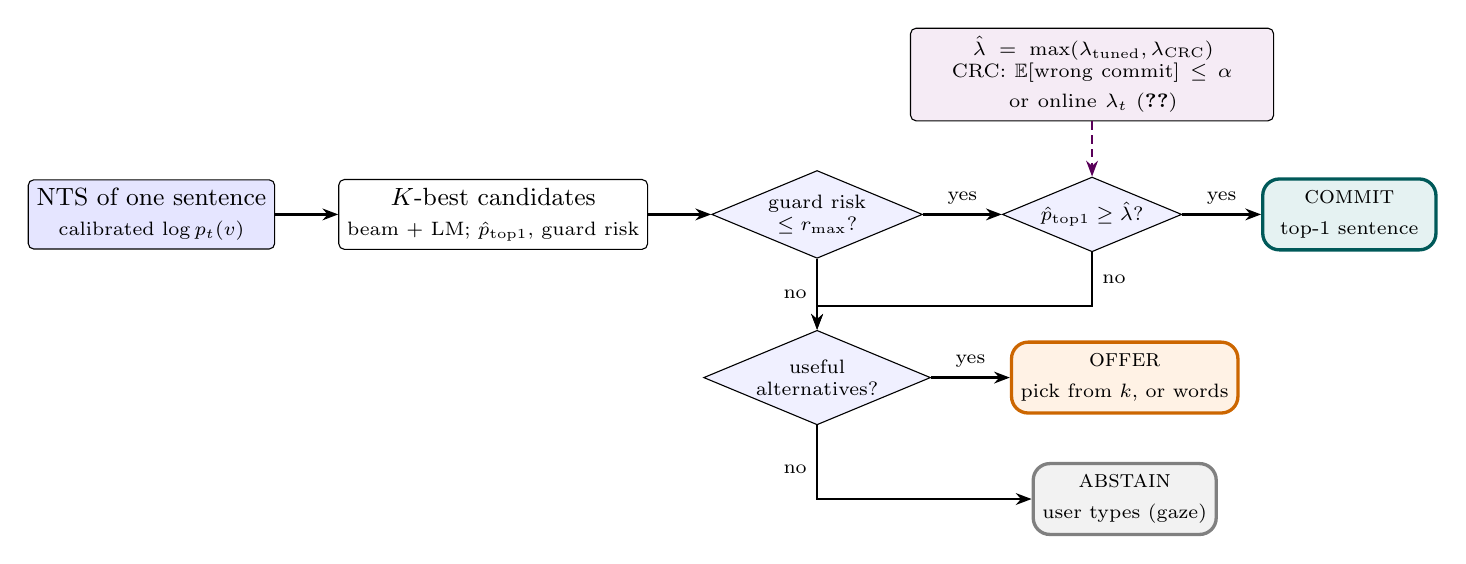
\begin{tikzpicture}[
  font=\small,
  box/.style={draw, rounded corners=2pt, align=center, fill=white, minimum height=8mm, inner sep=3pt},
  dec/.style={draw, diamond, aspect=2.4, align=center, fill=blue!6, inner sep=1pt, font=\scriptsize},
  act/.style={draw, rounded corners=6pt, align=center, minimum width=22mm, minimum height=9mm, very thick},
  arr/.style={-{Stealth[length=2mm]}, thick},
  node distance=5mm and 8mm]
  \node[box, fill=blue!10] (in) {NTS of one sentence\\\scriptsize calibrated $\log p_t(v)$};
  \node[box, right=of in] (cand) {$K$-best candidates\\\scriptsize beam + LM; $\hat p_{\mathrm{top1}}$, guard risk};
  \node[dec, right=of cand] (g) {guard risk\\$\le r_{\max}$?};
  \node[dec, right=10mm of g] (lam) {$\hat p_{\mathrm{top1}} \ge \hat\lambda$?};
  \node[act, draw=teal!70!black, fill=teal!10, right=10mm of lam] (commit) {\textsc{commit}\\\scriptsize top-1 sentence};
  \node[dec, below=9mm of g] (off) {useful\\alternatives?};
  \node[act, draw=orange!80!black, fill=orange!10, right=10mm of off] (offer) {\textsc{offer}\\\scriptsize pick from $k$, or words};
  \node[act, draw=gray, fill=gray!10, below=6mm of offer] (abst) {\textsc{abstain}\\\scriptsize user types (gaze)};
  \node[box, fill=violet!8, above=7mm of lam, text width=44mm] (thr) {\scriptsize $\hat\lambda = \max(\lambda_{\mathrm{tuned}}, \lambda_{\mathrm{CRC}})$\\\scriptsize CRC: $\mathbb{E}[\text{wrong commit}] \le \alpha$\\\scriptsize or online $\lambda_t$ (\cref{sec:online})};
  \draw[arr] (in) -- (cand);
  \draw[arr] (cand) -- (g);
  \draw[arr] (g) -- node[above, font=\scriptsize] {yes} (lam);
  \draw[arr] (lam) -- node[above, font=\scriptsize] {yes} (commit);
  \draw[arr] (g) -- node[left, font=\scriptsize] {no} (off);
  \draw[arr] (lam) |- node[pos=0.25, right, font=\scriptsize] {no} ($(off.north)+(0,3mm)$) -- (off.north);
  \draw[arr] (off) -- node[above, font=\scriptsize] {yes} (offer);
  \draw[arr] (off) |- node[pos=0.3, left, font=\scriptsize] {no} (abst);
  \draw[arr, violet!70!black, densely dashed] (thr.south) -- (lam.north);
\end{tikzpicture}
\end{adjustbox}
  \caption{\textbf{Trust decision for one item} (primary rule). A candidate is committed only if the guard (input-validity check) accepts it and its calibrated confidence reaches $\hat\lambda = \max(\lambda_{\mathrm{tuned}}, \hat\lambda_{\mathrm{LTT}})$. LTT bounds the risk over the mix of sessions that the calibration data come from. Otherwise the layer offers alternatives or abstains, and the user types with the fallback keyboard.}
  \label{fig:decision}
\end{figure}

\section{User-model variants and baselines}
\label{app:user}

Each variant changes one group of parameters of \cref{tab:user} and refits every policy: fallback speed 10 or 40 characters per minute (main 20); all selection, scanning, word-selection and navigation times scaled by 0.5 or 2; miss probability of a wrong committed word 0 or 0.2 (main 0.05). In the \emph{symmetric-offer} variants, an offer without the intended sentence makes the user fix the closest candidate word by word, missing each wrong word with the same probability as after a commit; full retyping is disabled. In the \emph{misspecified} evaluation, policies fitted under the main user are scored under each variant without refitting; they lost at most 0.2 \ewpm{} against refitting, except with symmetric offers and miss probability 0.2 on the weak decoders (MEG 1.18 vs 2.75).

\paragraph{Gaze typing with word completion.} The user types letter by letter at the fallback speed. Before each letter, the keyboard shows the three most frequent vocabulary words (counts $\ge 2$) that start with the typed prefix; there is no sentence context. If the intended word is shown and selecting it is faster, the user selects it at the scan-and-select cost for three slots plus the word-selection time. The main baseline charges no time for looking at the list, which favours it \citep{koester1994wordprediction}. Clinical AAC uses stronger, context-dependent prediction, so a realistic AAC baseline would probably be faster. Gaze typing with completion reached 5.84 (B2T '25), 6.19 (sEMG) and 4.10 (MEG) \ewpm{} (point values).

\paragraph{Always commit against the layer.} \Cref{tab:um} gives the paired difference per variant (plug-in layer, refitted).

\begin{table}[H]
  \centering
  \caption{\textbf{Trust layer minus always commit} (\ewpm{}, 95\% cluster-bootstrap CI), all policies refitted under each user-model variant. Values below 0: always commit is faster.}
  \label{tab:um}
  \scriptsize
  \begin{adjustbox}{max width=\linewidth}\begin{tabular}{@{}lllllll@{}}
    \toprule
    \inputrows{generated/tab_um_commit_head.tex}
    \midrule
    \inputrows{generated/tab_um_commit.tex}
    \bottomrule
  \end{tabular}\end{adjustbox}
\end{table}

\section{Decoder quality}
\label{app:decoders}

Excluding the 6 MEG test sentences with a close training variant (CER $\le 0.25$ to a training sentence) gave 0.519 (greedy) and 0.492 (beam), so memorisation of near variants explains at most 0.02 of the CER. On sEMG, plain key accuracies (0.299, 0.168, 0.209) are below the majority-class rate (space, 0.338) because the CNNs rarely predict space; balanced accuracy is the fair metric. Over three MEG seeds, the greedy CER was 0.254, 0.243 and 0.140 below the shuffled control of the same seed (\cref{tab:seeds}). For context, the published asynchronous MEG encoder reports a CER of $0.59 \pm 0.02$ with another split and without key-time training labels \citep{zhang2026brain2qwertyv2}.

\begin{table}[H]
  \centering
  \caption{\textbf{Decoder quality and input controls (test sets).} Exact: share of items whose top-1 sentence is right; in $K$-best: share whose intended sentence is in the 10-best list. MEG: the trust harness keeps an insertion bonus of 1.0 tuned on raw streams; the validation-tuned bonus of 0 gives the 0.475 row. ``---'': not applicable or not computed.}
  \label{tab:decoders}
  \small
  \begin{adjustbox}{max width=\linewidth}\begin{tabular}{@{}lllll@{}}
    \toprule
    \textbf{Device / decoder} & \textbf{CER} & \textbf{WER} & \textbf{Exact / in $K$-best} & \textbf{Controls and floors} \\
    \midrule
    MEG, asynchronous, greedy & 0.506 & 0.842 & --- & shuffled 0.760, zeros 0.925 \\
    MEG, beam + LM tuned on validation & 0.475 & 0.809 & 0.005 / --- & text-only floor 0.688 \\
    MEG, beam in the trust harness & 0.522 & --- & 0.003 / 0.016 & --- \\
    \midrule
    B2T '25, our phoneme-to-word decoder & 0.095 & 0.149 & 0.390 / 0.623 & --- \\
    B2T '25, published decoder & 0.031 & 0.043 & 0.806 / --- & --- \\
    \midrule
    sEMG keys: accuracy (balanced) & \multicolumn{2}{l}{0.299 (0.367) / 0.168 (0.240) / 0.209 (0.226)} & --- & permuted labels 0.022 (0.032) \\
    sEMG sentences after LM & 0.123 / 0.398 / 0.479 & 0.214 / 0.579 / 0.681 & 0.459 / 0.118 / 0.038 & in $K$-best 0.64 / 0.21 / 0.08 \\
    \bottomrule
  \end{tabular}\end{adjustbox}
\end{table}

\begin{table}[H]
  \centering
  \caption{\textbf{MEG decoder over three training seeds} (637 test instances; trust harness fitted on validation). Seed 0 is the paper's decoder.}
  \label{tab:seeds}
  \small
  \begin{adjustbox}{max width=\linewidth}\begin{tabular}{@{}lllll@{}}
    \toprule
    & \textbf{Seed 0} & \textbf{Seed 1} & \textbf{Seed 2} & \textbf{Mean $\pm$ SD} \\
    \midrule
    Test CER, greedy & 0.506 & 0.502 & 0.592 & $0.533 \pm 0.051$ \\
    Test CER, beam + LM (validation-tuned) & 0.475 & 0.467 & 0.567 & $0.503 \pm 0.056$ \\
    Shuffled MEG, greedy & 0.760 & 0.745 & 0.732 & $0.746 \pm 0.014$ \\
    Zero input, greedy & 0.925 & 0.948 & 0.819 & $0.897 \pm 0.069$ \\
    Always commit: \ewpm{} / wrong-commit & 2.58 / 0.997 & 2.55 / 0.994 & 2.35 / 1.000 & \\
    Trust: \ewpm{} / commits & 3.20 / 0 & 3.16 / 0 & 2.96 / 0 & \\
    Trust $-$ gaze (gaze 3.15) & \ci{-0.11}{+0.26} & \ci{-0.15}{+0.23} & \ci{-0.30}{-0.05} & \\
    Eligible to commit / truth in 10-best & 0.024 / 0.016 & 0.036 / 0.019 & 0.002 / 0.000 & \\
    \bottomrule
  \end{tabular}\end{adjustbox}
\end{table}

\section{Per-device settings}
\label{app:settings}

The policy grid has 1,980 points: commit threshold $\lambda \in \{0.3$, 0.4, 0.5, 0.6, 0.7, 0.8, 0.85, 0.9, 0.95, 0.98, $1.01\}$; maximum guard risk for a commit $r_{\max} \in \{0.1$, 0.2, 0.3, 0.5, $1.0\}$; offer limit $k_{\max} \in \{0$, 1, 2, 3, 5, $8\}$; abstain risk $r_{\mathrm{abst}} \in \{0.6, 0.8, 1.01\}$; and fallback $\in \{$offer, abstain$\}$. $\tau_s$ reached the upper end of its search interval (20, which flattens the confidence) on MEG and sEMG cross-subject. Decoder settings are in the experiment configurations in the repository.

\begin{table}[H]
  \centering
  \caption{\textbf{Per-device settings of the shared trust-layer implementation} (full-fit pipeline; fitted on each device's fit data, MEG: validation set). Max.\ guard risk: largest guard risk that still allows a commit.}
  \label{tab:settings}
  \small
  \begin{adjustbox}{max width=\linewidth}\begin{tabular}{@{}lllll@{}}
    \toprule
    & \textbf{MEG} & \textbf{B2T '25, ours} & \textbf{B2T '25, published gate} & \textbf{sEMG (cal.\ / x-sess.\ / x-subj.)} \\
    \midrule
    Frame temperature $\tau_f$ & 3.30 & 3.78 & 3.78 & 1.25 / 1.78 / 2.17 \\
    Sentence temperature $\tau_s$ & 20.0 & 4.56 & 1.72 & 2.42 / 5.42 / 20.0 \\
    LM weight (beam) & 0.5 (insertion bonus 1.0) & 1.0 (word LM; edit penalty 12, word bonus 3) & as ours & 1.0 / 1.0 / 1.5 \\
    Candidate list $K$ & 10 & 10 & published sentence + our 10 (bonus +2.0) & 10 \\
    Plug-in commit threshold & 0.5 & 0.5 & 0.7 & 0.7 / 0.3 / 0.3 \\
    Max.\ guard risk for commit & 0.3 & 0.5 & 0.5 & 1.0 / 1.0 / 0.1 \\
    Offer size $k$ & 1 & 2 & 1 & 2 / 2 / 1 \\
    Guard & \multicolumn{4}{l}{low-evidence threshold 0.5; consistency over the top 5; risk $=\max$(low evidence, 1 $-$ consistency)} \\
    \bottomrule
  \end{tabular}\end{adjustbox}
\end{table}

\section{All policies on the fixed test sets}
\label{app:full}

\paragraph{Why the fit-A rows differ from the full-fit plug-in row.} In the two fixed splits, the fall from 0.059 (full fit) to 0.025 (split A) came entirely from the policy grid chosen on fit-A (commit threshold 0.3 and maximum guard risk 0.1, against 0.5 and 0.5 on the full fit data): the full-fit temperatures with the fit-A policy also gave 0.0245. In split A, CRC and LTT were not binding (CRC's calibration bound at the chosen threshold was 0.0075); in split B, the fit-A policy (threshold 0.4, guard 0.3) gave 0.060, and the risk control removed correct commits. Over random re-splits, the CRC max rule changed the plug-in decisions in 54\% (ours) and 34\% (published) of re-splits. Pure CRC on split A stops at the lowest eligible calibration score (0.3075); test items below it are never committed, which is why pure CRC (20 wrong) is stricter than LTT at $\lambda = 0$ (22 wrong).

\paragraph{Per day, plug-in layer.} The plug-in layer beat always offering on 12 of 13 days with a difference (ours; sign test $p = 0.003$) and 14 of 14 (published; $p = 0.0001$); against always committing it tied (7 of 14 days; $p = 1.0$) and lost on 13 of 14 days (published).

\begin{table}[H]
  \centering
  \caption{\textbf{More policies on the fixed test sets.} Columns as in \cref{tab:main}. Plain threshold: full fit, no guard. Pure CRC / LTT: fit-A pipeline, clean calibration (B2T split A, $n = 401$; sEMG 143; MEG 199 instances of 5 sentences, no guarantee for new sentences), without the max rule. 256 non-templated: sEMG test sentences without a near variant in the LM text (\cref{app:leakage}). Unified bootstrap ($B = 2000$, seed 20261112).}
  \label{tab:full}
  \small
  \begin{adjustbox}{max width=\linewidth}\begin{tabular}{@{}lllllll@{}}
    \toprule
    \textbf{Device} & \textbf{Policy} & \textbf{\ewpm{} [CI]} & \textbf{Wrong-commit [CI]} & \textbf{Commit} & \textbf{EAC} & \textbf{Silent} \\
    \midrule
    B2T '25, ours & plain threshold (full fit) & 11.51 \ci{10.79}{12.35} & 0.036 \ci{0.025}{0.046} & 0.17 & 0.22 & 0 \\
     & CRC, pure (split A) & 11.48 \ci{10.79}{12.29} & 0.025 \ci{0.015}{0.035} & 0.10 & 0.24 & 0.001 \\
     & LTT, pure (split A) & 11.48 \ci{10.79}{12.29} & 0.027 \ci{0.016}{0.038} & 0.10 & 0.26 & 0.001 \\
    B2T '25, published & plain threshold (full fit) & 18.62 \ci{17.01}{20.17} & 0.025 \ci{0.014}{0.038} & 0.38 & 0.06 & 0.001 \\
     & CRC, pure (split A) & 18.79 \ci{17.13}{20.37} & 0.048 \ci{0.029}{0.071} & 0.49 & 0.10 & 0.005 \\
     & LTT, pure (split A) & 18.65 \ci{17.04}{20.20} & 0.029 \ci{0.013}{0.050} & 0.40 & 0.07 & 0.001 \\
    sEMG session-cal. & always offer & 8.01 \ci{6.92}{9.17} & 0 & 0 & --- & 0 \\
     & trust, plug-in & 8.02 \ci{6.93}{9.19} & 0.004 \ci{0}{0.009} & 0.04 & 2/21 & 0 \\
     & CRC, pure & 8.07 \ci{6.98}{9.26} & 0.040 \ci{0.025}{0.056} & 0.24 & 0.17 & 0.005 \\
     & LTT, pure & 8.04 \ci{6.97}{9.21} & 0.022 \ci{0.009}{0.036} & 0.18 & 0.12 & 0.002 \\
     & trust, 256 non-templated & 6.97 \ci{5.94}{8.09} & 0.004 (1/256) & 0.01 & 1/2 & 0 \\
    sEMG cross-session & always offer & 4.67 \ci{4.19}{5.25} & 0 & 0 & --- & 0 \\
     & CRC, pure & 4.66 \ci{4.18}{5.24} & 0.056 \ci{0.039}{0.074} & 0.09 & 0.61 & 0.007 \\
     & LTT, pure & 4.67 \ci{4.18}{5.25} & 0.031 \ci{0.021}{0.042} & 0.05 & 0.57 & 0.005 \\
     & trust, 256 non-templated & 4.08 \ci{3.77}{4.42} & 0 & 0 & --- & 0 \\
    sEMG cross-subject & LM weight re-tuned & 4.84 \ci{4.28}{5.51} & 0.002 \ci{0}{0.006} & 0.01 & 1/6 & 0 \\
     & trust, 256 non-templated & 3.69 \ci{3.50}{3.92} & 0 & 0 & --- & 0 \\
    MEG & CRC, pure (instance level) & 3.20 \ci{3.01}{3.43} & 0.028 \ci{0.006}{0.061} & 0.03 & 18/19 & 0.005 \\
     & LTT, pure (instance level) & 3.20 \ci{3.01}{3.44} & 0 & 0.002 & 0/1 & 0 \\
    \bottomrule
  \end{tabular}\end{adjustbox}
\end{table}

\section{Time-ordered tests: all designs and rules}
\label{app:forward}

Order inside a day is file order (the only time order in the data file). For each prefix of days, the pipeline is fitted on all trials of the fit days (the fit-A recipe) and item tables are built for every later day. \Cref{tab:forward-full} gives every design and rule, with and without the guard. Applying the V1 threshold 2--12 days later kept the LTT max rate near 0.02--0.03 on average (repository table). The plug-in rule had one day with a CP lower bound above $\alpha$ in V1 (day 46), V4 (day 48) and V3 (day 34) on our decoder.

\begin{table}[H]
  \centering
  \caption{\textbf{Time-ordered tests, all designs} (Brain-to-Text '25). Each cell: test days above $\alpha$ / test days, pooled wrong-commit rate (pooled commit rate). V1: calibrate on the previous day; V4: on the two previous days; V2: fit on days 1--3, calibrate on all earlier days; V3: calibrate on the first half of the test day.}
  \label{tab:forward-full}
  \scriptsize
  \begin{adjustbox}{max width=\linewidth}\begin{tabular}{@{}llllllll@{}}
    \toprule
    \textbf{Condition} & \textbf{Design} & \textbf{Plug-in} & \textbf{CRC pure} & \textbf{CRC max} & \textbf{LTT max} & \textbf{Joint $\beta{=}0.10$} & \textbf{Joint $\beta{=}0.20$} \\
    \midrule
    \inputrows{generated/tab_forward_full.tex}
    \bottomrule
  \end{tabular}\end{adjustbox}
\end{table}

\section{Per-day risk under the primary rule}
\label{app:perday}

\Cref{tab:perday} gives the LTT max wrong-commit rate per day. On the published gate, day 34 was above $\alpha$ in 94\% of re-splits; CRC max gave 0.108 and the plug-in rule 0.110 on that day. Joint LTT with $\beta = 0.10$ gave 0.016 on day 34 at a commit rate of 0.060. On sEMG, per test participant, LTT max stayed at or below 0.038 (session-calibrated), 0.023 (cross-session) and 0 (cross-subject). Per-day (Mondrian) LTT with a quarter of a day as calibration (8--52 items) was feasible only for day 76 (52 items $\ge 45$) and committed nothing on the other 13 days.

\begin{table}[H]
  \centering
  \caption{\textbf{Per-day wrong-commit rate, LTT max rule} (Brain-to-Text '25, guard on). Random re-splits: pooled over re-splits (5th--95th percentile), and share of re-splits with a day rate above $\alpha$. Fixed splits: wrong commits / test trials of the day. Bold: pooled rate above $\alpha$.}
  \label{tab:perday}
  \scriptsize
  \begin{adjustbox}{max width=\linewidth}\begin{tabular}{@{}llllllllll@{}}
    \toprule
    & & \multicolumn{2}{c}{\textbf{Ours, 50 re-splits}} & \multicolumn{3}{c}{\textbf{Published, re-splits}} & \textbf{Ours} & \multicolumn{2}{c}{\textbf{Published}} \\
    \cmidrule(lr){3-4}\cmidrule(lr){5-7}\cmidrule(lr){8-8}\cmidrule(lr){9-10}
    \textbf{Day} & \textbf{$n_{\mathrm{test}}$} & \textbf{Pooled} & $\boldsymbol{>\alpha}$ & \textbf{Pooled, 50 (p05--p95)} & $\boldsymbol{>\alpha}$ & \textbf{Pooled, 200} & \textbf{Split A} & \textbf{Split A} & \textbf{Split B} \\
    \midrule
    \inputrows{generated/tab_perday.tex}
    \bottomrule
  \end{tabular}\end{adjustbox}
\end{table}

\section{Random re-splits: sEMG rows and population risk}
\label{app:population}

\begin{table}[H]
  \centering
  \caption{\textbf{Random re-splits, sEMG and reuse rows} (50; guard on). Columns as in \cref{tab:repeat}. sEMG repeats keep the 551 test sentences fixed, so their spread is fit and calibration variation only. Cross-session: 34\% of re-splits never committed under the max rules, so the means mix zero-commit and committing re-splits. Cross-subject never committed under the max rules. Reused: pure CRC calibrated on the data that also fitted the pipeline.}
  \label{tab:repeat-full}
  \small
  \begin{adjustbox}{max width=\linewidth}\begin{tabular}{@{}llllll@{}}
    \toprule
    \textbf{Condition} & \textbf{Rule} & \textbf{Wrong-commit} & $\boldsymbol{>\alpha}$ \textbf{[CP95]} & \textbf{Commit} & \textbf{EAC} \\
    \midrule
    sEMG session-cal. & plug-in & 0.015 (0.004--0.033) & 0 \ci{0}{0.07} & 0.12 & 0.13 \\
     & CRC, pure & 0.029 (0.011--0.061) & 0.06 \ci{0.01}{0.17} & 0.19 & 0.15 \\
     & CRC, max rule & 0.013 (0.004--0.024) & 0 \ci{0}{0.07} & 0.11 & 0.12 \\
     & LTT, pure & 0.017 (0.009--0.034) & 0 \ci{0}{0.07} & 0.14 & 0.13 \\
     & \textbf{LTT, max rule} & 0.011 (0.004--0.019) & 0 \ci{0}{0.07} & 0.09 & 0.12 \\
    sEMG cross-session & plug-in & 0.008 (0--0.033) & 0.04 \ci{0}{0.14} & 0.02 & 0.44 \\
     & CRC, pure & 0.025 (0--0.063) & 0.14 \ci{0.06}{0.27} & 0.04 & 0.58 \\
     & CRC, max rule & 0.007 (0--0.027) & 0 \ci{0}{0.07} & 0.02 & 0.41 \\
     & LTT, pure & 0.017 (0--0.044) & 0.02 \ci{0}{0.11} & 0.03 & 0.53 \\
     & \textbf{LTT, max rule} & 0.006 (0--0.023) & 0 \ci{0}{0.07} & 0.02 & 0.38 \\
    B2T '25 ours & CRC, pure, reused & 0.055 (0.037--0.085) & 0.58 & 0.21 & 0.26 \\
    B2T '25 published & CRC, pure, reused & 0.050 (0.032--0.073) & 0.48 & 0.48 & 0.10 \\
    \bottomrule
  \end{tabular}\end{adjustbox}
\end{table}

\paragraph{Population risk.} LTT bounds the population risk at the chosen threshold, not the test rate of a finite split. A random split of a finite pool does not give that risk: the pool rate includes the calibration items on which the threshold was chosen (biased low), and the held-out rate adds test-sampling noise. If calibration sets are drawn \emph{with replacement} from the pool, the pool is the exact population of an i.i.d.\ draw, and its risk at the chosen threshold is known. On the test pools of 816 trials (2,000 draws, $n_{\mathrm{cal}} = 408$), the population risk of pure LTT exceeded $\alpha$ in 4.7\% \ci{3.8}{5.7} (ours) and 4.1\% \ci{3.3}{5.1} (published) of draws, within $\delta = 0.1$; pure CRC exceeded it in 37\% and 38\%, which CRC does not promise to avoid, while its mean population risk stayed at or below $\alpha$ (0.047--0.048). The pool-including-calibration design of an earlier version of this analysis (0.5\% and 1.5\%) is biased low; it gives 1.1\% and 0.9\% with 2,000 draws, and the held-out design gives 15\% and 12\%. For the random re-splits, with 200 with-replacement draws per re-split from that re-split's calibration and test pool, the population exceedance of LTT max was 0.026 (ours) and 0.014 (published); with 200 re-splits, 0.020 and 0.016, and the test-set exceedance 15/200 = 0.075 \ci{0.043}{0.121} and 11/200 = 0.055 \ci{0.028}{0.096}. LTT max was never above $\alpha$ in a re-split where CRC max was not (exact McNemar, 50 re-splits: 0 vs 3 discordant, $p = 0.25$, and 0 vs 6, $p = 0.031$; 200 re-splits: $p = 4.8 \times 10^{-7}$ and $1.2 \times 10^{-7}$).

\paragraph{CRC and LTT on random splits of the test pool.} Random calibration/test splits of the test pool are exchangeable by construction, so they check the implementation, not the assumption. \Cref{tab:crc} and \cref{fig:crc} give CRC and LTT at several calibration sizes. With 20 calibration trials, CRC kept the mean valid but never committed in 17\% of splits; LTT cannot commit below 45 items. A session-start block of the first 20 trials of each day gave CRC rates of 0.009 (ours) and 0.025 (published) at commit rates of 0.04 and 0.32, and 6 of 14 days never committed.

\begin{table}[H]
  \centering
  \caption{\textbf{CRC and LTT on random calibration/test splits of the test pool} ($\alpha = 0.05$, $\delta = 0.1$; 500 splits). Wrong-commit: mean test rate; p90: its 90th percentile; $P_{>\alpha}$: share of splits with a test rate above $\alpha$; Err.\,$|$\,commit: pooled over splits; Never: share of splits without a commit. MEG: pool of 637 instances (no guarantee for new sentences).}
  \label{tab:crc}
  \small
  \begin{adjustbox}{max width=\linewidth}\begin{tabular}{@{}llllllll@{}}
    \toprule
    \textbf{Data} & \textbf{Method, $n_{\mathrm{cal}}$} & \textbf{Wrong-commit} & \textbf{p90} & $\boldsymbol{P_{>\alpha}}$ & \textbf{Commit} & \textbf{Err.\,$|$\,commit} & \textbf{Never} \\
    \midrule
    B2T '25, our decoder & CRC, 20 & 0.0308 & 0.089 & 0.22 & 0.123 & 0.25 & 0.17 \\
     & CRC, 100 & 0.0456 & 0.075 & 0.38 & 0.186 & 0.25 & 0 \\
     & CRC, 408 & 0.0479 & 0.069 & 0.43 & 0.192 & 0.25 & 0 \\
     & LTT, 50 & 0.0201 & 0.046 & 0.09 & 0.097 & 0.21 & 0 \\
     & LTT, 408 & 0.0356 & 0.052 & 0.15 & 0.156 & 0.23 & 0 \\
    B2T '25, published gate & CRC, 408 & 0.0495 & 0.071 & 0.46 & 0.484 & 0.10 & 0 \\
     & LTT, 408 & 0.0355 & 0.054 & 0.15 & 0.429 & 0.08 & 0 \\
    MEG, asynchronous & CRC, 408 & 0.0197 & 0.031 & 0 & 0.021 & 0.93 & 0 \\
     & LTT, 408 & 0.0220 & 0.031 & 0 & 0.024 & 0.93 & 0 \\
    \bottomrule
  \end{tabular}\end{adjustbox}
\end{table}

\begin{figure}[H]
  \centering
  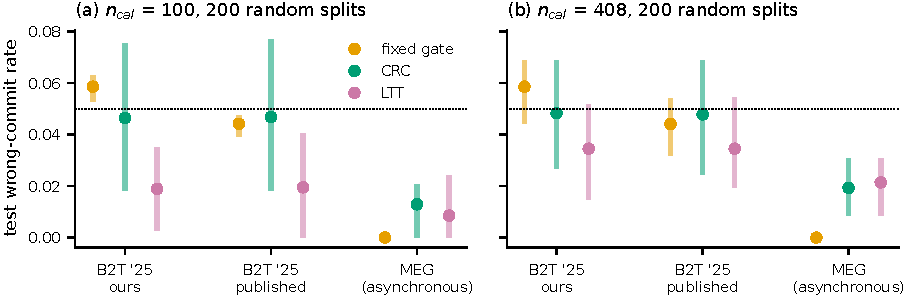
\includegraphics[width=\linewidth]{fig_crc_splits.pdf}
  \caption{\textbf{CRC bounds the mean over splits; LTT bounds the population risk with probability $1 - \delta$} (full-fit pipeline). Test wrong-commit rate over 200 random calibration/test splits of the test pool with (a)~100 and (b)~408 calibration items. Dots: mean; bars: 5th to 90th percentile. Dotted line: $\alpha = 0.05$. A test rate above $\alpha$ in a single split is not a violation of either guarantee.}
  \label{fig:crc}
\end{figure}

\section{Published-gate bonus}
\label{app:bonus}

The gate puts the published sentence on top of our $K$-best list with score = our best score + bonus (\code{published\_margin} in \code{experiments/2026-11-10-b2t25-trust/config.json}). The value 2.0 came with the first commit of that experiment (\code{3fb8154}, 2026-11-10) and never changed; no grid, tuning stage or selection record exists. The data file holds the published sentence but no scores or logits of the published decoder. With the published sentence as the only candidate (score 0, no character confidences), the layer has no signal to rank trials: the fitted policy never commits (threshold 1.01) and every rule equals always offering (18.11 \ewpm{}). Bonus 0 makes the published sentence tie with our top candidate; the layer then commits less and is 1.3 \ewpm{} slower.

\begin{table}[H]
  \centering
  \caption{\textbf{Sensitivity to the published-gate bonus} (guard on). Full fit: plug-in wrong-commit [day-cluster CI], commit, \ewpm{}. Splits A, B: LTT max wrong-commit (commit). Re-splits (50): LTT max mean wrong-commit, share above $\alpha$ (commit).}
  \label{tab:bonus}
  \small
  \begin{adjustbox}{max width=\linewidth}\begin{tabular}{@{}lllllll@{}}
    \toprule
    \textbf{Bonus} & \textbf{Full fit: wrong-commit} & \textbf{Commit} & \textbf{\ewpm{}} & \textbf{Split A} & \textbf{Split B} & \textbf{Re-splits} \\
    \midrule
    \inputrows{generated/tab_bonus.tex}
    \bottomrule
  \end{tabular}\end{adjustbox}
\end{table}

\section{Calibration and the commit trade-off}
\label{app:ece}

\begin{table}[H]
  \centering
  \caption{\textbf{Sentence calibration and error detection} (full-fit pipelines, fixed test sets; 95\% percentile bootstrap at the primary unit). ECE: 15 equal-width bins; the binned ECE is biased upwards, so a percentile interval can lie beside its point value. AUROC: positive class = wrong top-1 sentence. $^{a}$MEG: 2 of 637 top-1 sentences are right, so its AUROC is not informative.}
  \label{tab:ece}
  \small
  \begin{adjustbox}{max width=\linewidth}\begin{tabular}{@{}lllllll@{}}
    \toprule
    \textbf{Condition} & $\boldsymbol{n}$ & \textbf{Top-1 acc.} & \textbf{ECE raw} & \textbf{ECE calibrated} & \textbf{AUROC $1-\hat p$} & \textbf{AUROC guard} \\
    \midrule
    \inputrows{generated/tab_ece.tex}
    \bottomrule
  \end{tabular}\end{adjustbox}
\end{table}

\begin{figure}[H]
  \centering
  \begin{subfigure}[t]{0.32\linewidth}
    \centering
    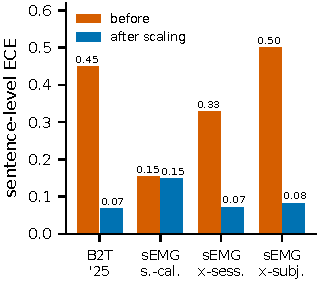
\includegraphics[width=\linewidth]{fig_ece.pdf}
    \caption{Sentence-level ECE.}
    \label{fig:ece}
  \end{subfigure}\hfill
  \begin{subfigure}[t]{0.33\linewidth}
    \centering
    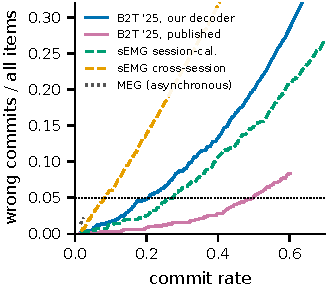
\includegraphics[width=\linewidth]{fig_risk_coverage.pdf}
    \caption{Marginal risk.}
    \label{fig:risk}
  \end{subfigure}\hfill
  \begin{subfigure}[t]{0.33\linewidth}
    \centering
    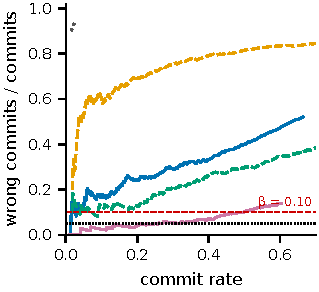
\includegraphics[width=\linewidth]{fig_selective_risk.pdf}
    \caption{Error among commits.}
    \label{fig:selrisk}
  \end{subfigure}
  \caption{\textbf{Calibration and the commit trade-off} (full-fit plug-in pipeline, test sets; not the guaranteed rule). (a)~Sentence ECE before and after temperature scaling. (b)~For each commit threshold: share of test items committed (x) and committed wrongly (y); dotted line: $\alpha = 0.05$. (c)~Error among commits at the same thresholds; dashed line: $\beta = 0.10$. Items blocked by the guard are never committed. Curves start at 10 commits. The error among commits of our decoder falls to 0.1--0.2 only below about 10\% commits; that of the published decoder stays near or below 0.15.}
  \label{fig:calib}
\end{figure}

\section{Ablation}
\label{app:ablation}

\Cref{tab:ablation} refits each variant on the condition's fit data and scores it on the same test items. \emph{No calibration}: no temperature. \emph{Confidence only}: both temperatures fitted, but the beam decodes the raw stream. \emph{No sentence temperature}: the frame temperature is applied before the beam and the sentence calibrator is the identity. \emph{No conformal sets}: \act{offer} shows the fitted top $k$. \emph{LM weight re-tuned}: on sEMG, the LM weight is chosen on fit-A CER with the frame-calibrated streams; on MEG, the validation-tuned beam (3.14 instead of 3.20 \ewpm{}, also no commits). Without the sentence temperature, the wrong-commit rate on our intracortical decoder rose to 0.076 (paired \ci{+0.001}{+0.036}). Without the guard, it fell to 0.036 on our decoder (paired \ci{-0.035}{-0.011}; lower on 9 of 10 days with a difference, sign test $p = 0.021$) and to 0.025 on the published gate (\ci{-0.034}{-0.007}); its AUROC for a wrong top sentence (0.702) was below that of $\hat p_{\mathrm{top1}}$. On sEMG cross-subject, re-tuning the LM weight gave 4.84 \ci{4.28}{5.51} \ewpm{} at top-1 CER 0.360 (instead of 0.479).

\begin{table}[H]
  \centering
  \caption{\textbf{Unified ablation} (full fit; \ewpm{} / wrong-commit rate; point values; ``='': equal to trust).}
  \label{tab:ablation}
  \small
  \begin{adjustbox}{max width=\linewidth}\begin{tabular}{@{}lllllll@{}}
    \toprule
    \textbf{Variant} & \textbf{B2T '25 ours} & \textbf{B2T '25 published} & \textbf{sEMG s.-cal.} & \textbf{sEMG x-sess.} & \textbf{sEMG x-subj.} & \textbf{MEG} \\
    \midrule
    trust (as reported) & 11.55 / 0.059 & 18.77 / 0.044 & 8.02 / 0.004 & 4.68 / 0.004 & 4.08 / 0 & 3.20 / 0 \\
    no calibration & 11.57 / 0.071 & 18.73 / 0.043 & 8.15 / 0.045 & 4.75 / 0.013 & 4.76 / 0.005 & 3.04 / 0.005 \\
    confidence only (raw decoding) & 11.54 / 0.074 & 18.74 / 0.047 & 8.07 / 0.018 & 4.76 / 0.007 & 4.75 / 0 & 3.04 / 0 \\
    no sentence temperature & 11.50 / 0.076 & 18.66 / 0.032 & 8.11 / 0.040 & 4.67 / 0.018 & 4.07 / 0.044 & 3.20 / 0 \\
    no guard & 11.51 / 0.036 & 18.62 / 0.025 & = & = & = & = \\
    no conformal sets & 11.53 / 0.059 & = & 8.07 / 0.020 & = & = & = \\
    \act{offer\_words} off (small grid) & 11.25 / 0.032 & 18.62 / 0.025 & 7.98 / 0.004 & 4.64 / 0 & 4.08 / 0 & 3.20 / 0 \\
    \act{offer\_words} on (small grid) & 11.32 / 0.054 & 18.59 / 0.026 & 7.99 / 0.015 & 4.64 / 0.005 & 4.08 / 0 & 3.20 / 0 \\
    LM weight re-tuned & --- & --- & 8.02 / 0.004 & 4.73 / 0.013 & 4.84 / 0.002 & 3.14 / 0 \\
    gaze typing only & 4.08 & 4.08 & 4.27 & 4.27 & 4.27 & 3.15 \\
    \bottomrule
  \end{tabular}\end{adjustbox}
\end{table}

\section{Data reuse and the fixed-split drift tests}
\label{app:reuse}

\Cref{tab:reuse} gives all 12 reuse comparisons (reused minus clean calibration, test wrong-commit, paired by re-split). The Wilcoxon test over re-splits is valid only conditional on this pool of trials, because the re-splits overlap. The delete-a-day (or delete-a-participant) jackknife recomputes both thresholds without each cluster over all re-splits, so its standard error includes the overlap; it does not refit the pipeline. Holm corrects over the 12 comparisons. Only our decoder shows an effect after Holm (pure CRC and CRC max). With 200 re-splits, our decoder's pure-CRC effect is $+0.0032$ (jackknife Holm-adjusted $p = 0.17$). A single deployment detects a shift of 0.035 (our decoder), 0.038 (published) or 0.040--0.057 (sEMG) with 80\% power.

\begin{table}[H]
  \centering
  \caption{\textbf{Calibration on reused data: all 12 comparisons} (50 re-splits). Diff: mean of reused minus clean test wrong-commit. Wilcoxon over re-splits (conditional on the pool; Holm-adjusted in brackets); sign: re-splits with reused higher / lower; jackknife 95\% CI and $p$ (Holm).}
  \label{tab:reuse}
  \scriptsize
  \begin{adjustbox}{max width=\linewidth}\begin{tabular}{@{}lllllll@{}}
    \toprule
    \textbf{Condition} & \textbf{Rule} & \textbf{Diff} & \textbf{Wilcoxon $p$ (Holm)} & \textbf{Sign} & \textbf{Jackknife CI} & \textbf{Jackknife $p$ (Holm)} \\
    \midrule
    \inputrows{generated/tab_reuse.tex}
    \bottomrule
  \end{tabular}\end{adjustbox}
\end{table}

\paragraph{Fixed-split drift tests.} On the fixed splits (\cref{tab:drift}), clean CRC gave 0.0245 and 0.0600 on our decoder, against 0.0625 when the full-fit pipeline was calibrated on its own fit data. The two clean values above $\alpha$ were within the range of exchangeable splits ($p = 0.21$ and $0.30$). In split A the test rate was above the exchangeable reference ($p = 0.012$; day-stratified $p = 0.014$) but below $\alpha$, where CRC was not binding; after Holm correction over the six tests, none was significant (split A: 0.072). These tests have low power: the 5th--95th percentile range of the reference is 0.029--0.071 on split B and the published gate, and 0.014--0.022 on split A. We claim neither within-day drift nor that reuse caused the old value of 0.0625.

\begin{table}[H]
  \centering
  \caption{\textbf{Fixed splits: clean vs reused calibration} (pure CRC; test sets). Bound: CRC calibration bound $(n\hat R_n(\hat\lambda)+1)/(n+1)$. Exch.\ ref.: mean (5th--95th percentile) over 1,000 random splits of the pooled calibration and test items; $p = (k+1)/(B+1)$, one-sided; Holm over the six tests.}
  \label{tab:drift}
  \small
  \begin{adjustbox}{max width=\linewidth}\begin{tabular}{@{}llllllll@{}}
    \toprule
    \textbf{Data ($n_{\mathrm{test}}$)} & \textbf{Reused} & \textbf{Clean CRC [CI]} & \textbf{Bound} & \textbf{Exch.\ ref.} & $\boldsymbol{p}$ & \textbf{Holm} & \textbf{LTT, pure} \\
    \midrule
    B2T '25 ours, split A (816) & 0.0625 & 0.0245 \ci{0.015}{0.035} & 0.0075 & 0.018 (0.014--0.022) & 0.012 & 0.072 & 0.0270 \\
    B2T '25 ours, split B (816) & 0.0625 & 0.0600 \ci{0.049}{0.071} & 0.0498 & 0.049 (0.029--0.071) & 0.21 & 1.0 & 0.0515 \\
    B2T '25 published, split A (816) & 0.0490 & 0.0478 \ci{0.029}{0.071} & 0.0498 & 0.049 (0.029--0.074) & 0.54 & 1.0 & 0.0294 \\
    B2T '25 published, split B (816) & 0.0490 & 0.0490 \ci{0.030}{0.073} & 0.0498 & 0.050 (0.031--0.074) & 0.50 & 1.0 & 0.0306 \\
    sEMG cross-session (551) & 0.0635 & 0.0563 \ci{0.039}{0.074} & 0.0486 & 0.045 (0.018--0.080) & 0.30 & 1.0 & 0.0309 \\
    sEMG session-cal.\ (551) & 0.0417 & 0.0399 \ci{0.025}{0.056} & 0.0486 & 0.047 (0.018--0.082) & 0.60 & 1.0 & 0.0218 \\
    \bottomrule
  \end{tabular}\end{adjustbox}
\end{table}

\section{Online re-calibration}
\label{app:online}

An online controller re-tunes the commit threshold from user feedback, with a long-run guarantee for any sequence of items (\cref{tab:online}). On the fixed splits (warm start on the clean calibration data, then the test data in file order), the online controllers kept the long-run rate at 0.0245--0.0527 (Brain-to-Text '25) and 0.0381--0.0526 (sEMG), at \ewpm{} within 0.06 of offline CRC (\cref{tab:online-results}). The bounds say nothing about short windows: the largest rate in a rolling window of 50 items was 0.06--0.18. When only noticed errors were fed back (delay 10), \texttt{aci} reached 0.027--0.058 while its certificate on the observed losses was at most 0.0509: silent errors look correct to the controller. The sEMG online order is participant by participant, not a time sequence.

\begin{table}[H]
  \centering
  \caption{\textbf{Online re-calibration methods.} $L_t$: realised loss of item $t$; $T$: items in the sequence; $d$: feedback delay. The \texttt{aci} variants bound the long-run average of the \emph{observed} losses for any sequence; \texttt{window} and \texttt{decay} have no guarantee under shift.}
  \label{tab:online}
  \small
  \begin{adjustbox}{max width=\linewidth}\begin{tabular}{@{}llll@{}}
    \toprule
    \textbf{Method} & \textbf{Update} & \textbf{Guarantee} & \textbf{Feedback} \\
    \midrule
    \texttt{window} & CRC on the last $N = 200$ items with known truth & none under shift & full \\
    \texttt{decay} & weighted CRC on all past items, weights $0.99^{\text{age}}$ & none under shift & full \\
    \texttt{aci} & $\lambda_{t+1} = \max(0, \lambda_t + \eta(L_t - \alpha))$, $\eta = 0.05$ \citep{gibbs2021aci,angelopoulos2023pid,feldman2023rolling} & $\frac1T\sum_t L_t \le \alpha + \frac{\lambda_{T+1} - \lambda_1}{\eta T}$; a priori $\alpha + \frac{1 - \lambda_1 + \eta(1+d)}{\eta T}$ & realised only \\
    \texttt{aci\_window} & window CRC at level $\alpha_t$; $\alpha_{t+1} = \min(2\alpha, \alpha_t + \gamma(\alpha - L_t))$, $\gamma = 0.005$ & $\frac1T\sum_t L_t \le \alpha + \frac{\alpha_1 - \alpha_{T+1}}{\gamma T}$ & full + realised \\
    \bottomrule
  \end{tabular}\end{adjustbox}
\end{table}

\begin{table}[H]
  \centering
  \caption{\textbf{Online re-calibration on the fixed splits} (long-run test wrong-commit rate). Cert.\ / a priori: \texttt{aci} bound after the fact and in advance.}
  \label{tab:online-results}
  \small
  \begin{tabular}{@{}llllll@{}}
    \toprule
    \textbf{Data} & \texttt{window} & \texttt{decay} & \texttt{aci} & \texttt{aci\_window} & \textbf{Cert.\ / a priori} \\
    \midrule
    B2T '25 ours, split A & 0.0245 & 0.0257 & 0.0270 & 0.0245 & 0.043 / 0.068 \\
    B2T '25 ours, split B & 0.0478 & 0.0453 & 0.0527 & 0.0490 & 0.053 / 0.066 \\
    B2T '25 published, split A & 0.0429 & 0.0392 & 0.0478 & 0.0453 & 0.048 / 0.059 \\
    B2T '25 published, split B & 0.0441 & 0.0392 & 0.0478 & 0.0453 & 0.048 / 0.059 \\
    sEMG cross-session & 0.0472 & 0.0381 & 0.0526 & 0.0490 & 0.053 / 0.081 \\
    sEMG session-cal. & 0.0490 & 0.0454 & 0.0490 & 0.0490 & 0.049 / 0.072 \\
    \bottomrule
  \end{tabular}
\end{table}

\section{LM leakage check}
\label{app:leakage}

A near variant is a sentence within a character edit distance of 0.25 times its length, after normalisation, in the 600,000-sentence training slice of the English character LM. Of the 1,717 unique Brain-to-Text '25 cue sentences, 22 have an exact copy and 310 an exact or near variant; of the 551 sEMG test sentences, none has an exact copy and 295 have a near variant (Tatoeba is heavily templated). Rebuilding the LMs without these sentences changed 2 of 1,628 top-1 sentences on Brain-to-Text '25 and sEMG trust \ewpm{} by at most $-0.04$, and no wrong-commit rate by more than 0.002. Rebuilding does not remove the advantage of templated test sentences, which are easier to decode, so we also scored the 256 sEMG test sentences without a near variant: trust \ewpm{} fell from 8.02, 4.68 and 4.08 to 6.97, 4.08 and 3.69; trust minus gaze typing became \ci{+1.82}{+3.92}, \ci{-0.37}{+0.27} and \ci{-0.66}{-0.23}; always-commit wrong-commit rates rose to 0.664, 0.961 and 0.992; and the layer stayed safe (1 wrong commit in 256 sentences; one-sided upper bound 0.018). On Brain-to-Text '25, excluding the 147 test trials with a near variant gave a trust wrong-commit rate of 0.055 (all: 0.059) on our decoder and 0.042 (0.044) on the published gate.

\section{MEG decoder and sentence-level limits}
\label{app:meg}

We split 19 participants' data by a hash of the sentence text into 101 training, 11 validation and 17 test sentences (637 test instances); the same people appear in all splits, and no test sentence is in training or LM text. All trust parameters are fitted on the 437 validation instances (6 sentences fit, 5 calibrate in the deployment protocol). The decoder is a convolutional front end (320 channels) followed by 4 Conformer layers of width 256 \citep{gulati2020conformer}, trained with CTC and a keystroke auxiliary loss that uses key times as training labels. At inference it takes the MEG segment (first key $-$ 0.4\,s to last key press $+$ 0.5\,s), its length and the participant index; it has no key input (the published asynchronous decoder takes the same inputs but uses no key-time labels \citep{zhang2026brain2qwertyv2}). The trust harness keeps the beam settings of the earlier harness; with the validation-tuned beam the layer also committed nothing.

\paragraph{Sentence-grouped calibration.} Instances of one sentence are dependent, so a guarantee for new sentences needs the sentence as the unit: sentence-level CRC needs at least 19 calibration sentences and LTT 45, while the data set has 5 clean calibration, 11 validation and 17 test sentences. Sentence-level CRC was therefore infeasible and never committed. With calibration and test sentences disjoint, instance-level CRC gave mean test rates of 0.016--0.019 (never above $\alpha$ in 1,000 splits each with 5, 8 or 11 calibration sentences), but only 2.4\% of instances were eligible and 0.91--0.94 of the commits were wrong; the max rule committed nothing. Two-way MEG intervals: trust minus gaze typing \ci{-0.10}{+0.25} (sentences \ci{-0.04}{+0.15}, participants \ci{-0.08}{+0.22}); gaze typing with word completion was faster \ci{-1.13}{-0.64}. A synchronous control decoder with oracle key times gave the same trust result; over trials (instead of sentences) its difference to gaze typing excluded 0, which shows how trial-level intervals overstate MEG gains.

\section{Stream format, standards and audit log}
\label{app:format}

\paragraph{Fields and rules.} Besides the log-probability array, frame times, vocabulary, vocabulary type (\code{char}, \code{key}, \code{phoneme}, \ldots) and blank index, optional fields give the frame period, latency, producer and a \code{meta} object with named key prefixes (\code{device.*}, \code{decoder.*}, \code{lm.*}, \code{calibration.*}, \code{adapter.*}). A field is interpreted as a probability only if the stream declares it as one in \code{calibration.*}. Raw signals and direct identifiers stay out of the stream. NWB \citep{rubel2022nwb}, BCI2000 and OpenViBE \citep{schalk2004bci2000,renard2010openvibe}, IEEE P2731 and P2794 \citep{ieeep2731,ieeep2794,eiber2021reporting} and decoder benchmarks \citep{jayaram2018moabb,banville2026neuralbench} each cover part of the stack; none defines a per-frame decoded-output format with confidence semantics.

\paragraph{Serialisations, conformance and adapters.} The reference serialisations are an NPZ file and a JSON Lines streaming form. A conformance suite runs 60 checks, each tied to a specification clause, at three cumulative levels (\emph{core}, \emph{trust-ready}, \emph{provenance}); it ships 52 golden test vectors, and the reference consumer passes all 52. The adapters have 412 (intracortical), 568 (sEMG) and 156 (MEG) physical lines of Python. Mapping the decoders into the stream needed no change to the frame core of v0.1, a Development release written by the same authors.

\begin{table}[H]
  \centering
  \caption{\textbf{Devices, data and streams.} All data sets are public.}
  \label{tab:devices}
  \small
  \begin{adjustbox}{max width=\linewidth}\begin{tabular}{@{}llll@{}}
    \toprule
    & \textbf{Intracortical (speech)} & \textbf{Forearm sEMG (keys)} & \textbf{MEG (typing)} \\
    \midrule
    Data set (licence) & B2T '25 copy task (CC0) & Toronto sEMG (CC BY 4.0) & SpanishBCBL (CC BY-NC 4.0) \\
    Participants & 1 (T15, ALS) & 19 (healthy typists) & 19 (healthy typists) \\
    Test unit & 816 trials, 14 days & 551 composed sentences & 637 instances of 17 sentences \\
    Decoder & published online RNN; own phoneme-to-word decoder & own CNN & own asynchronous ConvCTC \\
    Stream vocabulary & \code{phoneme} (CTC, 41 tokens) & \code{key} (W3C codes) & \code{char} (CTC) \\
    Frame & 80\,ms & one per key press & 40\,ms \\
    Commit decision tested? & yes & weakly (0--9\% committed) & no (no right top-1) \\
    \bottomrule
  \end{tabular}\end{adjustbox}
\end{table}

\begin{figure}[H]
  \centering
  \begin{adjustbox}{max width=0.85\linewidth}% System architecture of Fidetype (paper version of wiki/diagrams/06 and 07).
% Included from latex/sections/format.tex with \input.
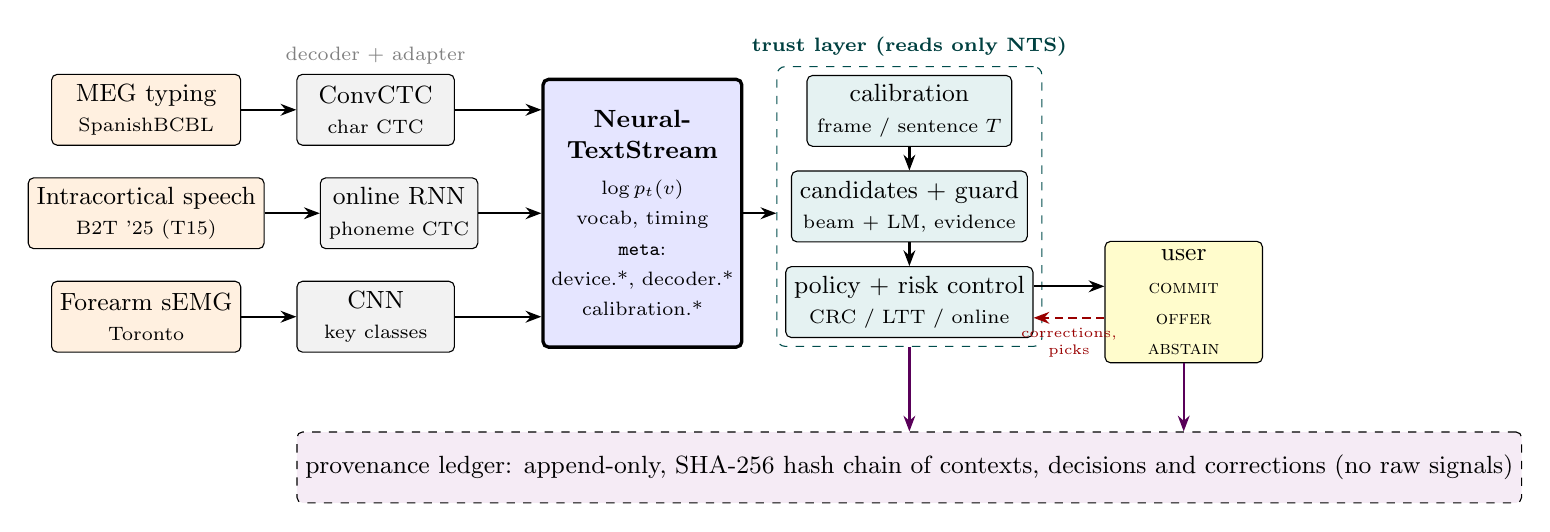
\begin{tikzpicture}[
  font=\small,
  box/.style={draw, rounded corners=2pt, align=center, minimum height=9mm, inner sep=3pt, fill=white},
  dev/.style={box, fill=orange!12, minimum width=24mm},
  ada/.style={box, fill=gray!10, minimum width=20mm},
  nts/.style={box, fill=blue!10, minimum width=22mm, minimum height=34mm, very thick},
  tl/.style={box, fill=teal!10, minimum width=26mm},
  usr/.style={box, fill=yellow!20, minimum width=20mm},
  led/.style={box, fill=violet!8, minimum width=118mm, dashed},
  arr/.style={-{Stealth[length=2mm]}, thick},
  fb/.style={-{Stealth[length=2mm]}, thick, densely dashed, red!60!black},
  node distance=4mm and 7mm]
  % devices
  \node[dev] (meg) {MEG typing\\\scriptsize SpanishBCBL};
  \node[dev, below=of meg] (ic) {Intracortical speech\\\scriptsize B2T '25 (T15)};
  \node[dev, below=of ic] (emg) {Forearm sEMG\\\scriptsize Toronto};
  % decoders + adapters
  \node[ada, right=of meg] (dmeg) {ConvCTC\\\scriptsize char CTC};
  \node[ada, right=of ic] (dic) {online RNN\\\scriptsize phoneme CTC};
  \node[ada, right=of emg] (demg) {CNN\\\scriptsize key classes};
  % NTS
  \node[nts, right=8mm of dic] (nts) {\textbf{Neural-}\\\textbf{TextStream}\\[2pt]\scriptsize $\log p_t(v)$\\\scriptsize vocab, timing\\\scriptsize \texttt{meta}:\\\scriptsize device.*, decoder.*\\\scriptsize calibration.*};
  % trust layer
  \node[tl, right=8mm of nts, yshift=13mm] (cal) {calibration\\\scriptsize frame / sentence $T$};
  \node[tl, below=3mm of cal] (cand) {candidates + guard\\\scriptsize beam + LM, evidence};
  \node[tl, below=3mm of cand] (pol) {policy + risk control\\\scriptsize CRC / LTT / online};
  \node[draw, rounded corners=3pt, dashed, teal!60!black, fit=(cal)(cand)(pol), inner sep=3pt, label={[teal!50!black,font=\scriptsize\bfseries]above:trust layer (reads only NTS)}] (tlbox) {};
  % user
  \node[usr, right=9mm of pol] (user) {user\\[1pt]\scriptsize \textsc{commit}\\\scriptsize \textsc{offer}\\\scriptsize \textsc{abstain}};
  % ledger
  \node[led, below=10mm of demg.south west, anchor=north west] (led) {provenance ledger: append-only, SHA-256 hash chain of contexts, decisions and corrections (no raw signals)};
  % arrows
  \foreach \a/\b in {meg/dmeg, ic/dic, emg/demg} \draw[arr] (\a) -- (\b);
  \foreach \a in {dmeg, dic, demg} \draw[arr] (\a.east) -- (\a.east -| nts.west);
  \node[font=\scriptsize, gray, above=0mm of dmeg] {decoder + adapter};
  \draw[arr] (nts.east) -- (nts.east -| tlbox.west);
  \draw[arr] (cal) -- (cand);
  \draw[arr] (cand) -- (pol);
  \draw[arr] ([yshift=2mm]pol.east) -- ([yshift=2mm]pol.east -| user.west);
  \draw[fb] ([yshift=-2mm]user.west) -- node[below, font=\tiny, align=center] {corrections,\\picks} ([yshift=-2mm]user.west -| pol.east);
  \draw[arr, violet!70!black] (tlbox.south) -- (tlbox.south |- led.north);
  \draw[arr, violet!70!black] (user.south) -- (user.south |- led.north);
\end{tikzpicture}
\end{adjustbox}
  \caption{\textbf{Architecture.} Each device's decoder emits a stream through a small adapter. The trust layer reads the stream: it calibrates confidence, builds candidate sentences, and chooses an action under a risk-control rule. The user's corrections and picks (dashed) can feed online re-calibration. Decisions can be written to a hash-chained audit log that stores no raw signals.}
  \label{fig:arch}
\end{figure}

\paragraph{Audit log.} Each decision can be appended to a JSON Lines log. Context entries are content-addressed and hold the adapter, decoder, LM, calibration and policy versions; decision entries hold the action, scores, a hash of the stream and its frame range; correction entries link to the decision they correct. Each entry stores the hash of the previous entry, so any edit, deletion or reordering breaks the chain; a separately stored head anchor detects truncation. The log stores no raw signals and is tamper-evident, not tamper-proof (no signature in v0). A replay of the 816 Brain-to-Text '25 test trials (1,723 entries) passed verification, recorded the same wrong commits as the harness, and detected every tampering case we tried, at about 0.1\,ms and 1.1\,kB per decision (\cref{fig:audit}).

\begin{figure}[H]
  \centering
  \fbox{\begin{minipage}{0.94\linewidth}\footnotesize\raggedright
  \textbf{Wrong commit} \texttt{dec-000041-ed60b4bd} (entry 44, hash \texttt{8cf2c6c67053b185...})\\
  Committed: ``who you never expect to when''\\
  Correction (known cue sentence, hash-linked): ``who you never expect to win''; 2 character edits, 1 word edit\\
  Scores: $\hat p_{\mathrm{top1}}$ 0.5814, set size 3, guard risk 0.2857; reason: $\hat p_{\mathrm{top1}} \ge 0.50$\\
  Input: stream \texttt{1b4b60e8e4950710...}, frames [0, 335], item \texttt{b2t25-test-trial-196}\\
  Decoder: published online RNN + our phoneme-to-word decoder; LM: Tatoeba character 6-gram + word unigram + CMUdict\\
  Calibration \texttt{cal-692fb52a73417552}: $\tau_f$ 3.7809, $\tau_s$ 4.5551; policy \texttt{pol-2eaa4ff51919527a}: commit threshold 0.5
  \end{minipage}}
  \caption{\textbf{One entry of the audit report} (B2T '25 replay, full-fit plug-in layer, our decoder; public CC0 copy-task cue, not the participant's own words). Hashes are shortened.}
  \label{fig:audit}
\end{figure}

\section{What each calibration set was and was not used for}
\label{app:separate}

Both guarantees need the parts that define $s_i$ (temperatures, conformal sets, guard and policy thresholds) to be fitted on data disjoint from the calibration items. Four exceptions remain. (1) Brain-to-Text '25, fixed splits: the word-decoder grid (LM weight, edit penalty, word bonus; 12 points) was tuned on a random 400 of the 812 fit trials, so 187 and 189 of the 401 calibration trials of splits A and B were in that tuning set; re-tuning on fit-A only selected the same setting in both splits. (2) Brain-to-Text '25, random re-splits and time-ordered tests: the same 400 trials are permuted into fit-A, calibration and test parts (about 100 into calibration and 200 into test per re-split); the re-tune check covers only the two fixed splits, so this overlap is not checked. The grid is small, so the bias is likely small. (3) MEG: the decoder checkpoint was selected by validation CER, and the validation sentences include the 5 calibration sentences. (4) sEMG session-calibrated: calibration and test logits come from two cross-fitted decoder runs, so their score functions differ by design. LTT also needs i.i.d.\ sampling; our random splits sample without replacement from a finite pool, which makes its binomial test conservative.

\section{Controls}
\label{app:controls}

\Cref{tab:controls} gives the commits on the Brain-to-Text '25 control streams for the frozen configurations of drafts v3 and v4. With the guard, the split-A pipeline committed no frame-shuffled or uniform stream on either decoder, and its real-trial test rate was unchanged (0.0245 ours, 0.0294 published; a refit that reproduces the committed values). On Brain-to-Text '25, the guard risk separated frame-shuffled and uniform streams from real ones with AUROC 0.981 and 0.998. On MEG the layer committed nothing on real input either, so its zero commits on controls carry no information; the guard risk separated shuffled MEG, zero input and uniform streams (AUROC 0.92, 1.00, 1.00), but not frame-shuffled streams (0.47) (\cref{fig:null}c).

\begin{table}[H]
  \centering
  \caption{\textbf{Commits on the Brain-to-Text '25 control streams} (300 test trials; split-A pipeline unless marked). Other trial: the real stream of a different sentence (intent mismatch). Frame-shuffled and uniform streams carry no neural information, so every commit on them is wrong. Uniform WC: wrong-commit rate on uniform streams.}
  \label{tab:controls}
  \small
  \begin{adjustbox}{max width=\linewidth}\begin{tabular}{@{}lllllll@{}}
    \toprule
    \textbf{Decoder} & \textbf{Configuration} & \textbf{Real} & \textbf{Other trial} & \textbf{Frame-shuffled} & \textbf{Uniform} & \textbf{Uniform WC} \\
    \midrule
    \inputrows{generated/tab_controls.tex}
    \bottomrule
  \end{tabular}\end{adjustbox}
\end{table}

\begin{figure}[H]
  \centering
  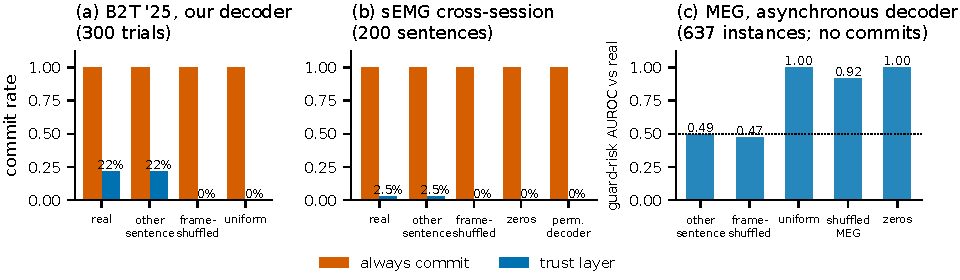
\includegraphics[width=\linewidth]{fig_null_audit.pdf}
  \caption{\textbf{Controls} (full-fit plug-in layer with the guard). (a, b)~Commit rate of always commit (orange) and the trust layer (blue) on real input, the intent-mismatch control (other sentence) and signal-destroying controls: (a)~B2T '25, our decoder, 300 test trials; (b)~sEMG cross-session, 200 test sentences. (c)~MEG, 637 instances: AUROC of the guard risk for separating each control from real input (dotted line: chance).}
  \label{fig:null}
\end{figure}

\section{How to state the guarantees}
\label{app:guarantees}

With LTT and the max rule (primary): ``if the calibration sentences and later sentences are i.i.d.\ draws from the same mix of sessions, and the calibration sentences fitted no other part of the system, then, with probability at least 0.9 over the choice of the calibration sentences, the long-run share of sentences committed wrongly, averaged over that mix of sessions, is at most 0.05''. It is not a statement about each session; in our data one day ran at about 0.10. With CRC: ``under exchangeability and the same separation, averaged over the choice of the $n$ calibration sentences and over a new sentence, the probability that the new sentence is committed wrongly is at most 0.05''; a single calibration set can exceed 0.05. With joint LTT: ``with probability at least 0.9, both the long-run wrong-commit share is at most $\alpha$ and the long-run share of wrong sentences among committed sentences is at most $\beta$'' (i.i.d.\ calibration sentences, separate from all fitted parts). With SGR: the bound of Geifman and El-Yaniv (2017, Theorem 3.2) on the error among accepted items, with probability at least 0.9, for i.i.d.\ calibration sentences separate from all fitted parts; its thresholds are chosen by bisection on the same data. With adaptive online re-calibration: ``for any sequence of sentences, the average observed wrong-commit rate over the first $T$ sentences is at most $0.05 + (1 - \lambda_1 + \eta(1+d))/(\eta T)$''. On MEG the unit is the sentence, and none of these statements applies to new sentences. All statements count only the errors that the system observes, so each should be reported with the measured silent-error rate.

\section{Data sets and licences}
\label{app:licences}

\begin{table}[H]
  \centering
  \caption{\textbf{Data sets, resources and licences.}}
  \label{tab:licences}
  \small
  \begin{tabular}{@{}p{4.3cm}p{2.4cm}p{3.6cm}p{4.2cm}@{}}
    \toprule
    \textbf{Data set / resource} & \textbf{Licence} & \textbf{Use} & \textbf{Note} \\
    \midrule
    SpanishBCBL \citep{levy2026brain2qwerty,spanishbcbl} & CC BY-NC 4.0 & MEG decoder training and evaluation & Research only; weights trained on it are not released for commercial use \\
    Brain-to-Text '25 copy-task logits \citep{card2024accurate,card2025data} & CC0 1.0 & intracortical trust evaluation & Companion code has no licence; we wrote our own loader \\
    Toronto sEMG typing \citep{achituve2025emg,achituve2024data} & CC BY 4.0 & sEMG decoder and trust evaluation & Baseline code (CC BY-SA 4.0) not used \\
    Tatoeba English / Spanish sentences & CC BY 2.0 FR (some CC0) & character LMs; composed sEMG sentences & Sentences from Tatoeba (\url{https://tatoeba.org}), by the Tatoeba contributors \\
    CMUdict (commit 7479086) & BSD-2-Clause style & phoneme-to-word lexicon & Copyright notice kept \\
    Brain2Qwerty code (Meta) & CC BY-NC 4.0 & read only, not copied & Our decoders are our own implementations \\
    Fidetype code and specification & Apache-2.0 & all methods & --- \\
    \bottomrule
  \end{tabular}
\end{table}


\bibliographystyle{unsrtnat}
\bibliography{refs}

\end{document}
